\documentclass[dvipdfmx,11pt]{beamer}

\usepackage{bxdpx-beamer}% dvipdfmxなので必要
\usepackage{listings,jlisting}%ソースコード貼り付けのため
\usepackage{tikz}
\usepackage{otf}
\usetikzlibrary{positioning}
\usetikzlibrary{shadows}
\AtBeginDvi{\special{pdf:tounicode 90ms-RKSJ-UCS2}} %% しおりが文字化けしないように
\setbeamertemplate{navigation symbols}{} %% 右下のアイコンを消す

\renewcommand{\kanjifamilydefault}{\gtdefault}

\usetheme{Warsaw}
%\usetheme{Darmstadt}

\setbeamertemplate{footline}[frame number] %% スライド下のバーを消してフレーム番号を表示
\useoutertheme{shadow}                 %% 箱に影をつける
\usefonttheme{professionalfonts}       %% 数式の文字を通常の LaTeX と同じにする

\usepackage{graphicx,xcolor}%%文字の色
%\usepackage{bm}
\usepackage{ipsj}
\usepackage{color}
\usepackage{amssymb}
\usepackage{amsmath}
\usepackage{amsthm}
\usepackage{multirow,bigdelim}
\newcommand{\la}{\leftarrow}
\newcommand{\Lra}{\Longrightarrow}
\newcommand{\Lla}{\Longleftarrow}
\newcommand{\Llra}{\Longleftrightarrow}
\newcommand{\lra}{\longrightarrow}
\newcommand{\dd}{\mathop{..}}
\newcommand{\range}[2]{\{#1\dd#2\}}
\newcommand{\imp}{\Rightarrow}
\newcommand{\equ}{\Leftrightarrow}
\renewcommand{\labelenumi}{(\arabic{enumi})}
\newcommand{\alldiff}{\textrm{alldifferent}}
\newcommand{\Alldiff}{\alldiff(x_1,x_2,\ldots,x_n)}
\newcommand{\SAT}{{\tt SAT}}
\newcommand{\UNSAT}{{\tt UNSAT}}
\newcommand{\Dom}{{\it Dom}}
% \newcommand{\p}[2]{p(#1,#2)}
\newcommand{\dE}[2]{p(#1=#2)}
\newcommand{\lE}[2]{p(#1^{(#2)})}
\newcommand{\oE}[2]{p(#1\le#2)}
 % 自分用のマクロ

\title{解集合プログラミングを用いた\\ハミルトン閉路問題の解法に関する考察}
\author{平手 貴大(101730309)}
\institute{名古屋大学情報学部コンピュータ科学科情報システム系\\番原研究室}
\date{2020年度 卒業研究発表会\\2021年2月19日}

\begin{document}
%%%%%%%%%%%%%%%%%%%%%%%%%%%%%%%%%%%%%%%%%%%%%%%%%%%%%%%%%%%%%%%%%%%

\frame{\maketitle}
%%%%%%%%%%%%%%%%%%%%%%%%%%%%%%%%%%%%%%%%%%%%%%%%%%%%%%%%%%%%%%%%%%%

\begin{frame}{ハミルトン閉路問題(Hamiltonian Cycle Problem)}
  \begin{itemize}
  \item \alert{ハミルトン閉路問題}
    \begin{itemize}
    \item 与えられたグラフの全頂点をちょうど一度ずつ
      通る閉路が存在するかどうかを判定する問題.
    \item 始点と終点が一致するという閉路の条件を
      取り除けば,ハミルトン路問題となる.
    \end{itemize}
  \item \alert{最短ハミルトン閉路問題}
    \begin{itemize}
    \item グラフの辺に距離が付随しているときに
      最短距離のハミルトン閉路を求める問題.
    \end{itemize}
  \item \alert{コスト制約付きハミルトン閉路問題}
    \begin{itemize}
    \item ハミルトン閉路問題に,距離の総和が所与の閾値以下
      (または以上)であることを制約条件として付加した問題.
    \end{itemize}
  \end{itemize}
  \begin{alertblock}{}
    本研究では,無向グラフ上のハミルトン閉路問題
    およびその関連問題を対象とする.    
  \end{alertblock}
\end{frame}
%%%%%%%%%%%%%%%%%%%%%%%%%%%%%%%%%%%%%%%%%%%%%%%%%%%%%%%%%%%%%%%%%%%

\begin{frame}{コスト制約付きハミルトン閉路問題}
%%%%%%%%%%%%%%%%%%%%%%%%%%%%%%%%%%%%%%%%%%%%%%%
  \begin{figure}[tb]
  \centering
  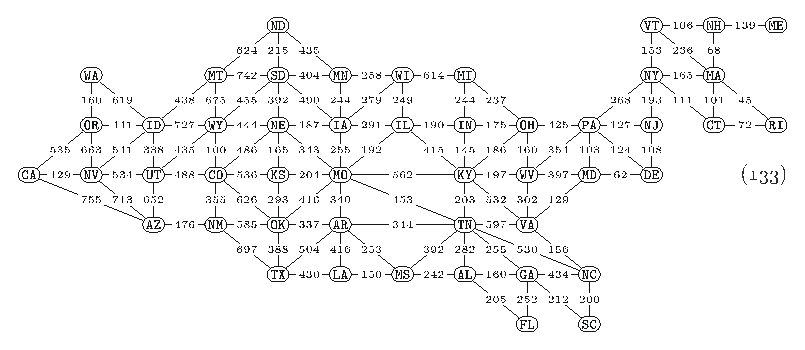
\includegraphics[width=0.8\linewidth]{fig/taocp_vol4fasc1b_p52_eq133.pdf}
%  \caption{D.~E.~Knuth の教科書にある最短ハミルトン路問題の例}
  \end{figure}
%%%%%%%%%%%%%%%%%%%%%%%%%%%%%%%%%%%%%%%%%%%%%%%
  WA から ME までの距離の総和がある閾値以下である
  ハミルトン路を求める問題.
  \begin{itemize}
  \item WA から ME までのハミルトン路は 6,876,928 通り
    あり,最短ハミルトン路は 11698 マイル.
  \item 閾値を最短距離の 10\%増 (12,868 マイル) とした場合,
    解の総数は 16180 個.
  \end{itemize}
   
\end{frame}
%%%%%%%%%%%%%%%%%%%%%%%%%%%%%%%%%%%%%%%%%%%%%%%%%%%%%%%%%%%%%%%%%%%

\begin{frame}{解集合プログラミング(Answer Set Programming; ASP)}
  \begin{itemize}
  \item \alert{ASP 言語}は,一階論理に基づく知識表現言語の一種.
  \item \alert{ASP システム}は,論理プログラムから
    安定モデル意味論に基づく解集合を計算するシステム.
  \item 近年,SAT 技術を応用した高速 ASP システムが開発され,
    スケジューリング,プランニング,システム生物学,システム検証,
    制約充足問題,制約最適化問題など様々な分野への実用的応用が急速に拡大している.
  \end{itemize}

  \begin{alertblock}{ハミルトン閉路問題に ASP を用いる利点}
    \begin{itemize}
    \item ASP 言語は表現力が高く,制約の記述が容易.
    \item 組み込みの非閉路制約を利用できる.
    \item 高速な解列挙.
    \end{itemize}
  \end{alertblock}
\end{frame}
%% %%%%%%%%%%%%%%%%%%%%%%%%%%%%%%%%%%%%%%%%%%%%%%%%%%%%%%%%%%%%%%%%%%%

\begin{frame}{研究目的}
  \begin{alertblock}{研究目的}
  ASP 技術を活用し,大規模なハミルトン閉路問題を
    効率よく解く手法を模索する.
  \end{alertblock}
  \begin{block}{研究内容}
    \begin{enumerate}
    \item \structure{ハミルトン閉路問題を解く3種類の ASP 符号化を考案.}
      \begin{itemize}
      \item 3つの符号化 \textsf{undirected}, \textsf{directed}, \textsf{acyclicity}.
      \item 最短ハミルトン閉路問題,コスト制約付きハミルトン閉路問題へ拡張.
      \end{itemize}
    \item \structure{既存のベンチマーク問題集を用いた評価実験.}
      \begin{itemize}
      \item  ベンチマーク問題は7種類,計517問.
      \item ハミルトン閉路問題に対する実験.
      \item 最短ハミルトン閉路問題に対する実験.
      \item コスト制約付きハミルトン路問題に対する実験.
      \end{itemize}
    \end{enumerate}
  \end{block}
\end{frame}
%%%%%%%%%%%%%%%%%%%%%%%%%%%%%%%%%%%%%%%%%%%%%%%%%%%%%%%%%%%%%%%%%%%

\begin{frame}{提案する ASP 符号化}
  \begin{block}{ハミルトン閉路問題の表現}
    与えられた無向グラフ$G= (V,E)$上に,以下の2つの制約を満たす
    部分グラフ$G'= (V,E')$が存在するか判定する問題.
    \begin{itemize}
    \item $G'$の各頂点の次数が2.(\alert{次数制約})
    \item $G'$が連結である.(\alert{連結制約})
    \end{itemize}
  \end{block}
  \begin{itemize}
  \item \alert{\textsf{undirected}符号化}
    \begin{itemize}
    \item ハミルトン閉路問題を次数制約と連結制約で簡潔に表現した符号化.
    \end{itemize}
  \item \alert{\textsf{directed}符号化}
    \begin{itemize}
    \item \textsf{undirected}符号化をベースに,与えられた無向グラフを
      有向グラフ化して解く符号化.
    \end{itemize}
  \item \alert{\textsf{acyclicity}符号化}
    \begin{itemize}
    \item \textsf{directed}符号化をベースに,連結制約に代わり
      部分閉路を禁止する制約を使用.
      \item 組み込み非閉路制約で,部分閉路を禁止する制約を簡潔に表現.
    \end{itemize}
  \end{itemize}
\end{frame}
%%%%%%%%%%%%%%%%%%%%%%%%%%%%%%%%%%%%%%%%%%%%%%%%%%%%%%%%%%%%%%%%%%%

\begin{frame}{実験概要}
  %%  提案した符号化の性能を評価するために実験を行った.
  以下では,提案した符号化の性能を評価するために行った2つの実験について説明する.
  \begin{itemize}
  \item \structure{比較する ASP 符号化}:
    \begin{itemize}
    \item \textsf{undirected}符号化
    \item \textsf{directed}符号化
    \item \textsf{acyclicity}符号化
    \end{itemize}
  \item \structure{対象とする問題}:
    \begin{enumerate}
    \item ハミルトン閉路問題
      \begin{itemize}
      \item \structure{制限時間}: 30分/問
      \item \structure{オプション}: \textit{trendy}
      \item \structure{ベンチマーク問題}:\\
        \textsf{color04},
        \textsf{complete},
        \textsf{knight},
        \textsf{tsplib},
        \textsf{grid},
        \textsf{random}
      \end{itemize}
    \item コスト制約付きハミルトン路問題(解の全列挙)
      \begin{itemize}
      \item \structure{制限時間}: 3時間/問
      \item \structure{オプション}: \textit{crafty}
      \item \structure{ベンチマーク問題}: \textsf{usmap} (閾値: 10問)
      \end{itemize}
    \end{enumerate}
  \item \structure{ASP システム}: \textit{clingo-5.4.0}
  \item \structure{実験環境}: Mac mini Intel Corei7 3.2GHz, 64GBメモリ
  \end{itemize}
\end{frame}
%%%%%%%%%%%%%%%%%%%%%%%%%%%%%%%%%%%%%%%%%%%%%%%%%%%%%%%%%%%%%%%%%%%

\begin{frame}{ハミルトン閉路問題の実験結果(解けた問題数)}
%%%%%%%%%%%%%%%%%%%%%%%%%%%%%%%%%%%%%%%%%%%%%%%
\begin{table*}[t]\footnotesize
  \centering
% \tabcolsep = 0.8mm
% \renewcommand{\arraystretch}{1.2}
  \begin{tabular}{lr||r|r|r}
    頂点数 & 問題数 & \textsf{undirected} & \textsf{directed} & \textsf{acyclicity}\\
   \hline
    $\:\:\:\:\:\,\, 0 \leq |V| < 1000$  & 171   & 156   & \textbf{171}   & 155  \\
    $1000 \leq |V| < 2000$  & 165   & 120   & \textbf{158}   & 124  \\
    $2000 \leq |V| < 3000$  & 177   & 125   & \textbf{162}   & 73   \\
    $3000 \leq |V| < 4000$  & 185   & 104   & \textbf{148}   & 42   \\
    $4000 \leq |V| < 5000$  & 128   & 92    & \textbf{104}   & 28   \\
    $5000 \leq |V| < 6000$  & 80    & 63    & \textbf{68}    & 23   \\
    $6000 \leq |V| < 7000$  & 55    & 39    & \textbf{43}    & 21   \\
    $7000 \leq |V| < 8000$  & 28    & 12    & \textbf{14}    & 5    \\
    $8000 \leq |V| < 9000$  & 10    & 2     & \textbf{5}     & 1    \\
    $9000 \leq |V| < 10000$ & 2     & \textbf{2}     & \textbf{2}     & 1    \\
   \hline
    合計 & 1001 & 715   & \textbf{875}   & 473  
  \end{tabular}
  \vskip .5em
  \caption{ハミルトン閉路問題: 解けた問題数}
  \label{sat_table}
\end{table*}
%label{sat_table}
%%%%%%%%%%%%%%%%%%%%%%%%%%%%%%%%%%%%%%%%%%%%%%%

\begin{itemize}
\item \textsf{S+U}では,\textsf{undirected} と \textsf{acyclicity} が,
  \textsf{directed} よりも2問多く解いた.
\item \textsf{SAT}では,\textsf{undirected} が,最も多くの問題を解いた.
\item \textsf{UNSAT}では,\textsf{directed} と \textsf{acyclicity} 符号化が,
  \textsf{undirected} より1問多く解いた.
\end{itemize}
\end{frame}
%%%%%%%%%%%%%%%%%%%%%%%%%%%%%%%%%%%%%%%%%%%%%%%%%%%%%%%%%%%%%%%%%%%

\begin{frame}{ハミルトン閉路問題の実験結果(カクタスプロット)}
%%%%%%%%%%%%%%%%%%%%%%%%%%%%%%%%%%%%%%%%%%%%%%%
\begin{figure}[tb]
\begin{center}
  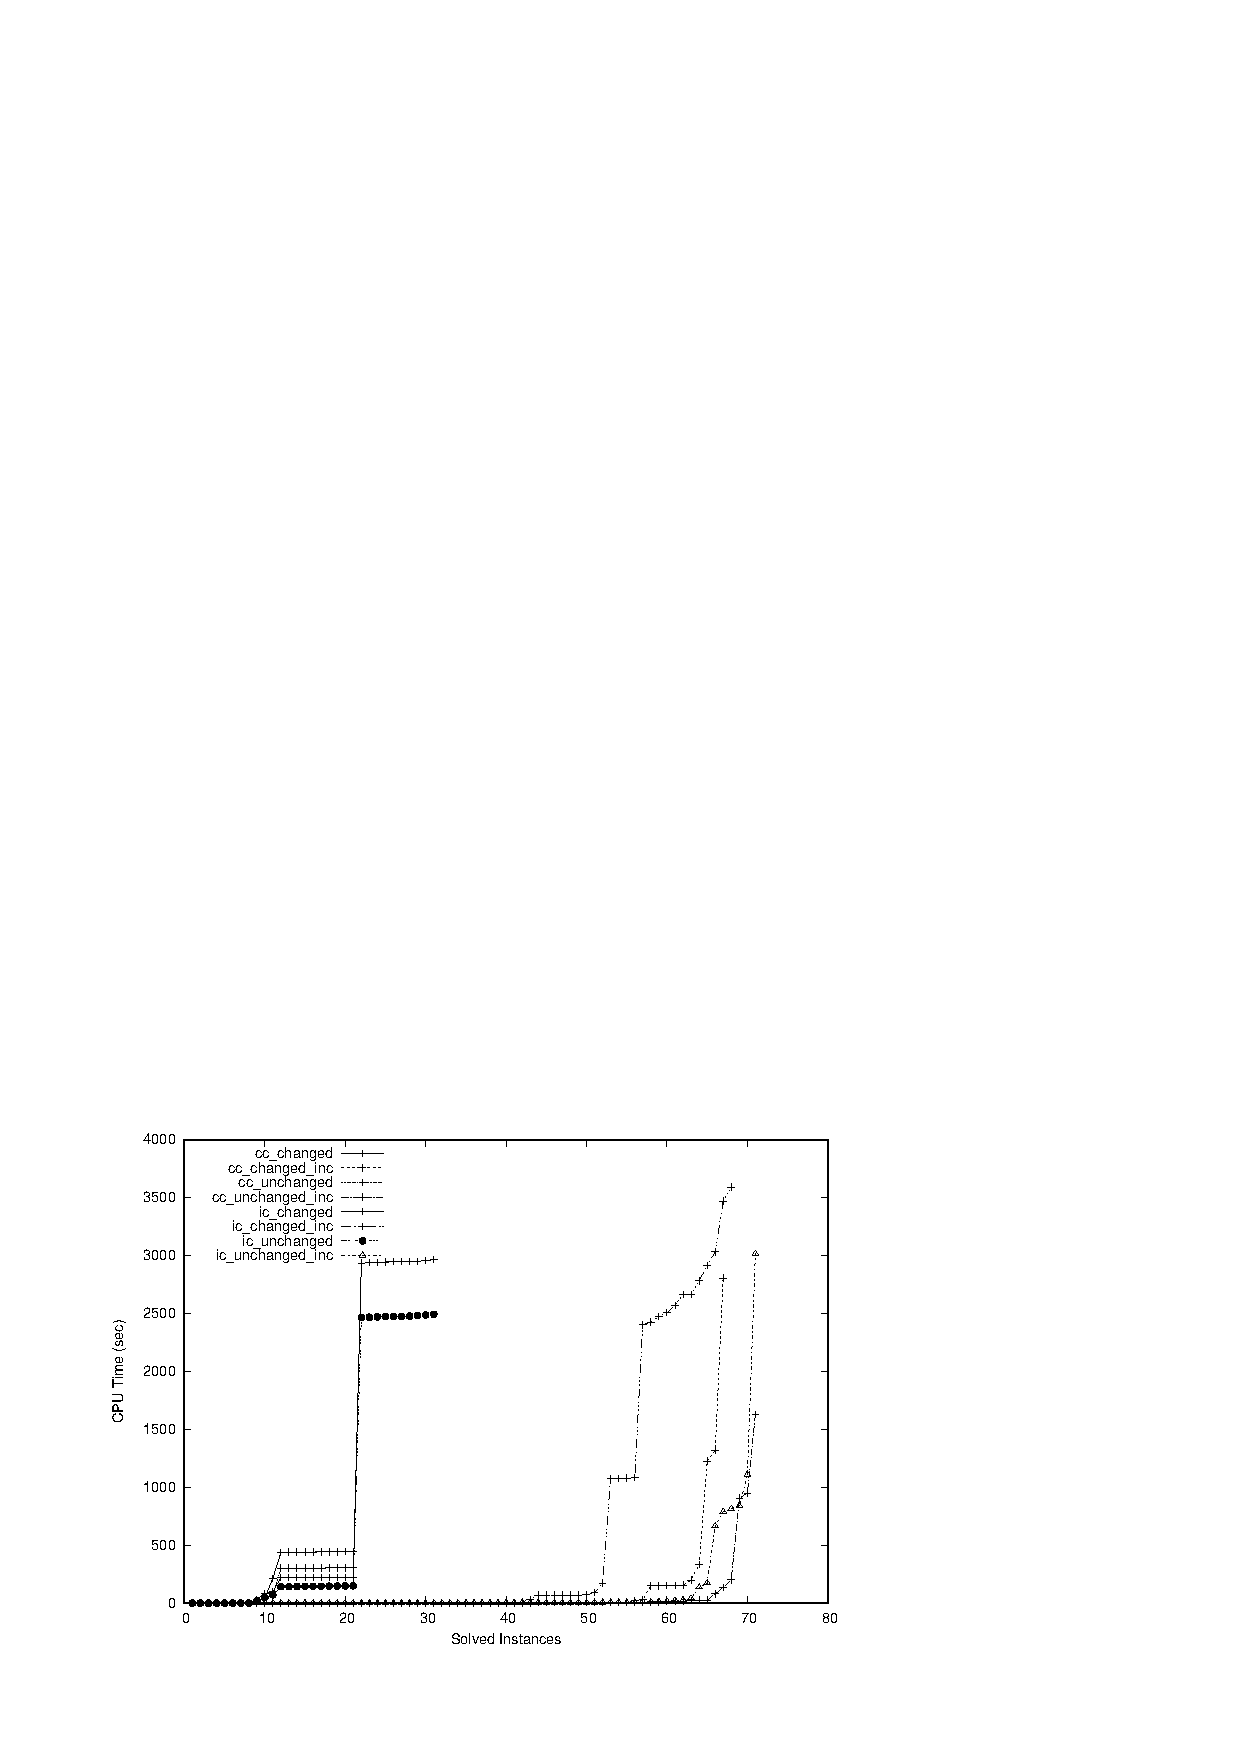
\includegraphics[width=0.7\linewidth]{fig/cactus.png}
%\caption{ハミルトン閉路問題: カクタスプロット (\textsf{SAT+UNSAT})}
\label{cactus}
\end{center}
\end{figure}
%%%%%%%%%%%%%%%%%%%%%%%%%%%%%%%%%%%%%%%%%%%%%%%

\begin{itemize}
\item \textsf{acyclicity}符号化は,
  解けた問題数が同じ\textsf{undirected}符号化と比較して,
  より高速に問題を解いていることが確認できた.
\end{itemize}
\end{frame}
%%%%%%%%%%%%%%%%%%%%%%%%%%%%%%%%%%%%%%%%%%%%%%%%%%%%%%%%%%%%%%%%%%%

\begin{frame}{コスト制約付きハミルトン路問題の実験結果}
%%%%%%%%%%%%%%%%%%%%%%%%%%%%%%%%%%%%%%%%%%%%%%%
\begin{table}[htbp]
  \caption{実験結果3}
  \label{cost_table}
  \centering
  \begin{tabular}{|l|r|rrr|}
    \hline
    制約Cost値    &	Models & undirected & directed & acyclicity \\
    \hline
    11698   &	1      &\textcolor{red}{2.919} &10.020 & 4.355	\\
    11814   &	8      &5.458  &7.416	& \textcolor{red}{4.136}	\\
    11931   &	28     &\textcolor{red}{3.226}&10.317	& 4.799	\\
    12282   &	388    &\textcolor{red}{9.993}&15.787	& 10.715	\\
    12867   &	16180  &16.386       &23.406	& \textcolor{red}{10.819}\\
    14037   &	939209 &47.894       &41.515	& \textcolor{red}{24.655}\\
    15207   &	4525541&85.256       &56.953	& \textcolor{red}{41.217}\\
    16377   &	6702964&93.595       &51.991	& \textcolor{red}{41.301}	\\
    17547   &	6876526&91.750       &46.065	& \textcolor{red}{37.290}	\\
    18716   &	6876928&95.659       &45.416	& \textcolor{red}{37.905}	\\
    \hline
    Average &   & 45.2136 & 30.889  & \textcolor{red}{21.7192}\\
    Best    &   & 3 & 0 & \textcolor{red}{7} \\
    \hline
  \end{tabular}
\end{table}
%\label{cost_table}
%%%%%%%%%%%%%%%%%%%%%%%%%%%%%%%%%%%%%%%%%%%%%%%

\begin{itemize}
\item \textsf{acyclicity}符号化が,より多くの問題を
  高速に解き,平均CPU時間も最も短かった.
\end{itemize}
    
\end{frame}
%%%%%%%%%%%%%%%%%%%%%%%%%%%%%%%%%%%%%%%%%%%%%%%%%%%%%%%%%%%%%%%%%%%

\begin{frame}{まとめ}
    \begin{enumerate}
    \item \structure{ハミルトン閉路問題を解く3種類の ASP 符号化を考案.}
      \begin{itemize}
      \item ASP の高い表現力による,最短ハミルトン閉路問題,コスト制約付きハミルトン閉路問題への自然な拡張.
      \end{itemize}
    \item \structure{既存のベンチマーク問題集を用いた評価実験.}
      \begin{itemize}
      \item ハミルトン閉路問題とコスト制約付きハミルトン路問題について,
        \textsf{acyclicity}符号化の優位性が確認できた.
      \item 最短ハミルトン閉路問題については,
        \textsf{undirected}符号化の優位性を確認した.(本発表では省略)
      \end{itemize}
    \end{enumerate}
  \begin{alertblock}{今後の課題}
    \begin{itemize}
    \item SATソルバーを用いた既存研究~\cite{soh14:jelia2014}で提案された,
      ハミルトン閉路問題をインクリメンタルに解く手法のASPを用いた実装.
    \item 巡回セールスマン問題への拡張.
    \end{itemize}
  \end{alertblock}
\end{frame}

%%%%%%%%%%%%%%%%%%%%%%%%%%%%%%%%%%%%%%%%%%%%%%%%%%%%%%%%%%%%%%%%%%%

\begin{frame}[noframenumbering]{}
  補足
\end{frame}
%%%%%%%%%%%%%%%%%%%%%%%%%%%%%%%%%%%%%%%%%%%%%%%%%%%%%%%%%%%%%%%%%%%

\begin{frame}[noframenumbering]{ベンチマーク詳細(1/2)}
\begin{itemize}
\item \textsf{color04} (127問)\\
  グラフ彩色問題の国際競技会
  COLOR02/03/04~\footnote{\url{https://mat.tepper.cmu.edu/COLOR02/}}
  で使用された問題インスタンス.
\item \textsf{complete} (15問)\\
  SATソルバーを用いた既存研究~\cite{soh14:jelia2014}で提供された
  完全グラフのインスタンス~\footnote{\url{https://tsoh.org/scarab/jelia2014/}}.
\item \textsf{knight} (11問)\\
%  \cite{DBLP:conf/sat/EenS03}で用いられた
  $N\times N$の騎士巡回問題(Knight's Tour)のインスタンス.\\
  $N=8,12,20,30,40,50,60,70,80,90,100$の11通り.
\item \textsf{tsplib} (9問)\\
  巡回セールスマン問題のポータルサイトTSPLIBに公開されている
  インスタンス\footnote{\url{http://comopt.ifi.uni-heidelberg.de/software/TSPLIB95/hcp/}}.
\end{itemize}  
\end{frame}
%%%%%%%%%%%%%%%%%%%%%%%%%%%%%%%%%%%%%%%%%%%%%%%%%%%%%%%%%%%%%%%%%%%

\begin{frame}[noframenumbering]{ベンチマーク詳細(2/2)}
\begin{itemize}
\item \textsf{grid} (12問)\\
  $N$次の正方グリッドグラフのインスタンス($6\leq N\leq 17$).
\item \textsf{random} (320問)\\
  SATソルバーを用いた既存研究~\cite{soh14:jelia2014}で提供された
  ランダムグラフのインスタンス~\footnote{\url{https://tsoh.org/scarab/jelia2014/}}.
\item \textsf{usmap} (1問)\\
  %図~\ref{fig:USmap}に示されたグラフ.
  D.~E~.Knuth の教科書
  The Art of Computer Programming~\cite{Knuth:TAOCP:SAT}
  に記載されている最短ハミルトン路問題の例.
\end{itemize}
\end{frame}
%%%%%%%%%%%%%%%%%%%%%%%%%%%%%%%%%%%%%%%%%%%%%%%%%%%%%%%%%%%%%%%%%%%

\begin{frame}[noframenumbering]{ベンチマークサイズ}
\begin{itemize}
\item \textsf{color04} (127問)\\
  辺の数: 11〜10000, 頂点の数: 20〜990000.
\item \textsf{complete} (15問)\\
  辺の数: 100〜1500, 頂点の数: 4950〜1124250.
\item \textsf{knight} (11問)\\
  辺の数: 64〜10000, 頂点の数: 168〜38808.
\item \textsf{tsplib} (9問)\\
  辺の数: 1000〜5000, 頂点の数: 1998〜9999.
\item \textsf{grid} (12問)\\
  辺の数: 36〜289, 頂点の数: 60〜544.
\item \textsf{random} (320問)\\
  辺の数: 100〜50000, 頂点の数: 319〜362828.
\item \textsf{usmap} (1問)\\
  辺の数: 48, 頂点の数:105 
\end{itemize}
\end{frame}
%%%%%%%%%%%%%%%%%%%%%%%%%%%%%%%%%%%%%%%%%%%%%%%%%%%%%%%%%%%%%%%%%%%

\begin{frame}[noframenumbering]{\textit{clingo} のオプション}
   \begin{itemize}
     \item [\textit{frumpy}] 以前の\textit{clasp}のバージョンで使用されていたものと同様の保守的なデフォルト.
     \item [\textit{jumpy}] より攻撃的なデフォルト.
     \item [\textit{tweety}] 典型的なASPの問題を想定したデフォルト.
     \item [\textit{trendy}] 構造的な問題を想定したデフォルト.
     \item [\textit{crafty}] 細工された問題を対象としたデフォルト.
     \item [\textit{handy}] 大規模な問題を対象としたデフォルト。
%     \item \<ファイル\>:\ 設定ファイルを使用してソルバーを設定する。
   \end{itemize}
\end{frame}
%%%%%%%%%%%%%%%%%%%%%%%%%%%%%%%%%%%%%%%%%%%%%%%%%%%%%%%%%%%%%%%%%%%

\begin{frame}[noframenumbering]{最短ハミルトン閉路問題の実験}
  \begin{itemize}
  \item \structure{比較する ASP 符号化}:
    \begin{itemize}
    \item \textsf{undirected}符号化
    \item \textsf{directed}符号化
    \item \textsf{acyclicity}符号化
    \end{itemize}
  \item \structure{制限時間}: 3時間/問
  \item \structure{オプション}: \textit{trendy}
  \item \structure{ベンチマーク問題}: \textsf{grid}と\textsf{usmap}
  \item \structure{ASP システム}: \textit{clingo-5.4.0}
  \item \structure{実験環境}: Mac mini Intel Corei7 3.2GHz, 64GBメモリ
  \end{itemize}
\end{frame}
%%%%%%%%%%%%%%%%%%%%%%%%%%%%%%%%%%%%%%%%%%%%%%%%%%%%%%%%%%%%%%%%%%%

\begin{frame}[noframenumbering]{最短ハミルトン閉路問題の実験結果}
%%%%%%%%%%%%%%%%%%%%%%%%%%%%%%%%%%%%%%%%%%%%%%%
\begin{table}[t]\footnotesize
  \caption{最短ハミルトン閉路問題: 得られた目的関数の値}
  \label{min_table_tr}
  \tabcolsep = 2mm
  %\renewcommand{\arraystretch}{1.0}
  \vskip .5em
  \centering
  \begin{tabular}{l|rrr}\hline
     問題 & \textsf{undirected} & \textsf{directed} & \textsf{acyclicity} \\
    \hline
    grid5&50,656*&50,656*&50,656* \\
    grid6&68,656*&68,656*&68,656* \\
    grid7&91,822*&91,822*&91,822* \\
    grid8&113,250&\textcolor{red}{112,916}&113,277 \\
    grid9&\textcolor{red}{142,502}&143,326&143,660 \\
    grid10&\textcolor{red}{172,703}&174,866&175,999 \\
    grid11&\textcolor{red}{200,399}&204,456&200,638 \\
    grid12&\textcolor{red}{231,278}&239,275&232,012 \\
    grid13&\textcolor{red}{276,692}&276,926&276,899 \\
    grid14&317,617&\textcolor{red}{317,144}&317,676 \\
    grid15&\textcolor{red}{375,906}&376,809&376,210 \\
    grid16&421,249&\textcolor{red}{419,737}&423,753 \\
    US48&11,698*&11,698*&11,698* \\
    \hline
    最適値と最良値の数 & 10 & 7 & 4\\    \hline
  \end{tabular}
\end{table}
%\label{min_table_tr}
%%%%%%%%%%%%%%%%%%%%%%%%%%%%%%%%%%%%%%%%%%%%%%%

\begin{itemize}
\item 最適値と最良値の数は,
\textsf{undirected}符号化が10問でもっとも多く,
その優位性が確認できた.
\end{itemize}
    
\end{frame}
%%%%%%%%%%%%%%%%%%%%%%%%%%%%%%%%%%%%%%%%%%%%%%%%%%%%%%%%%%%%%%%%%%%

\begin{frame}[noframenumbering]{ハミルトン閉路問題の実験考察}
%%%%%%%%%%%%%%%%%%%%%%%%%%%%%%%%%%%%%%%%%%%%%%%
\input{fig/cyclesat_table2.tex}%label{sat_table2}
%%%%%%%%%%%%%%%%%%%%%%%%%%%%%%%%%%%%%%%%%%%%%%%

%%%%%%%%%%%%%%%%%%%%%%%%%%%%%%%%%%%%%%%%%%%%%%%
\begin{table}[t]\tiny
%  \caption{ハミルトン閉路問題: 内訳考察}
  \label{difins_table}
  \centering  
  %\tabcolsep = 0.8mm
  \renewcommand{\arraystretch}{1.2}
  \begin{tabular}{lrr||rrr||rrr}
    問題 & 頂点数 & 辺の数 & \multicolumn{3}{c ||}{\textsf{undirected}} & \multicolumn{3}{c}{\textsf{acyclicity}}\\
    & & & variables & constraints & result & variables & constraints & result\\
    \hline
    \textsf{grid12} & 169 & 312 & 2079 & 2485 & UNKN & 962 & 2036 & \alert{UNSAT}\\
    \textsf{3-FullIns\_5} & 2030 & 33751 & 105280 & 141029 & \alert{SAT} & 71562 & 8256 & UNKN\\
  \end{tabular}
\end{table}
%label{difins_table}
%%%%%%%%%%%%%%%%%%%%%%%%%%%%%%%%%%%%%%%%%%%%%%%

\begin{itemize}
\item \textsf{grid12}については,変数の数において,
  \textsf{acyclicity}符号化が少ない値を示していたため,
  要するCPUtimeを短縮できたと考える.
\item \textsf{3-FullIns\_5}については,まだ考察中.
\end{itemize}
\end{frame}
%%%%%%%%%%%%%%%%%%%%%%%%%%%%%%%%%%%%%%%%%%%%%%%%%%%%%%%%%%%%%%%%%%%

\begin{frame}[noframenumbering]{ASP を用いたハミルトン閉路問題の解法}
%%%%%%%%
\begin{figure}[h]
  \centering
  \thicklines
  \setlength{\unitlength}{1.0pt}
  \small\footnotesize\scriptsize
  \begin{picture}(280,57)(4,-10)
    \put(  0, 20){\dashbox(50,24){\shortstack{HCP問題\\インスタンス}}}
    \put( 60, 20){\framebox(50,24){変換器}}
    \put(120, 20){\dashbox(50,24){\shortstack{ASPファクト}}}
    \put(120,-10){\dashbox(50,24){\shortstack{ASP符号化\\\tiny{(論理プログラム)}}}}
    \put(180, 20){\framebox(50,24){ASPシステム}}
    \put(240, 20){\dashbox(50,24){\shortstack{HCP問題\\の解}}}
    \put( 50, 32){\vector(1,0){10}}
    \put(110, 32){\vector(1,0){10}}
    \put(170, 32){\vector(1,0){10}}
    \put(230, 32){\vector(1,0){10}}
    \put(170, +2){\line(1,0){4}}
    \put(174, +2){\line(0,1){30}}
  \end{picture}  
%\caption{ASP を用いたハミルトン閉路問題(HCP)の解法}
\label{fig:arch}
\end{figure}
%%%%

\begin{itemize}
\item 与えられたハミルトン閉路問題は ASP ファクトに変換.
\item ASP ファクトはハミルトン閉路問題を解く ASP 符号化と結合.
\item ASP システムによって解が計算される.
\end{itemize}
\end{frame}
%%%%%%%%%%%%%%%%%%%%%%%%%%%%%%%%%%%%%%%%%%%%%%%%%%%%%%%%%%%%%%%%%%%

\begin{frame}[noframenumbering]{グラフの ASP ファクト}

%%%%%%%%%%%%%%%%%%%%%%%%%%%%%%
\begin{figure}[t]
\begin{center}
\begin{tikzpicture}
  %ノード1  
  \draw(4,2) circle (0.5)
  node[at={(4.1,2.1)}] {
    \begin{tabular}{c}
      1
    \end{tabular}
  };
  %ノード2  
  \draw(4,0) circle (0.5)
  node[at={(4.1,0.1)}] {
    \begin{tabular}{c}
      2
    \end{tabular}
  };
  %ノード3  
  \draw(6,2) circle (0.5)
  node[at={(6.1,2.1)}] {
    \begin{tabular}{c}
      3
    \end{tabular}
  };
  %ノード4  
  \draw(6,0) circle (0.5)
  node[at={(6.1,0.1)}] {
    \begin{tabular}{c}
      4
    \end{tabular}
  };
  %ノード5  
  \draw(8,2) circle (0.5)
  node[at={(8.1,2.1)}] {
    \begin{tabular}{c}
      5
    \end{tabular}
  };
  %ノード6  
  \draw(8,0) circle (0.5)
  node[at={(8.1,0.1)}] {
    \begin{tabular}{c}
      6
    \end{tabular}
  };
\draw(4,0.5) --(4,1.5);
\draw(6,0.5) --(6,1.5);
\draw(8,0.5) --(8,1.5);
\draw(4.5,0) --(5.5,0);
\draw(4.5,2) --(5.5,2);
\draw(6.5,0) --(7.5,0);
\draw(6.5,2) --(7.5,2);
\end{tikzpicture}

\end{center}
\end{figure}
%%%%%%%%%%%%%%%%%%%%%%%%%%%%%%

%%%%%%%%%%%%%%%%%%%%%%%%%%%%%%
\lstinputlisting[]{code/graph_example.lp}
%%%%%%%%%%%%%%%%%%%%%%%%%%%%%%

\end{frame}
%%%%%%%%%%%%%%%%%%%%%%%%%%%%%%%%%%%%%%%%%%%%%%%%%%%%%%%%%%%%%%%%%%%

\begin{frame}[noframenumbering]{\textsf{undirected} 符号化}

%%%%%%%%%%%%%%%%%%%%%%%%%%%%%%
\lstinputlisting[]{code/hamilton1.lp}
%%%%%%%%%%%%%%%%%%%%%%%%%%%%%%

\end{frame}
%%%%%%%%%%%%%%%%%%%%%%%%%%%%%%%%%%%%%%%%%%%%%%%%%%%%%%%%%%%%%%%%%%%

\begin{frame}[noframenumbering]{\textsf{directed} 符号化}

%%%%%%%%%%%%%%%%%%%%%%%%%%%%%%
\lstinputlisting[]{code/hamilton2.lp}
%%%%%%%%%%%%%%%%%%%%%%%%%%%%%%

\end{frame}
%%%%%%%%%%%%%%%%%%%%%%%%%%%%%%%%%%%%%%%%%%%%%%%%%%%%%%%%%%%%%%%%%%%

\begin{frame}[noframenumbering]{\textsf{acyclicity} 符号化}

%%%%%%%%%%%%%%%%%%%%%%%%%%%%%%
\lstinputlisting[]{code/hamilton3.lp}
%%%%%%%%%%%%%%%%%%%%%%%%%%%%%%

\end{frame}
%%%%%%%%%%%%%%%%%%%%%%%%%%%%%%%%%%%%%%%%%%%%%%%%%%%%%%%%%%%%%%%%%%%

\begin{frame}[noframenumbering]{符号化の拡張}
  
%%%%%%%%%%%%%%%%%%%%%%%%%%%%%%
\lstinputlisting[numbers=none]{code/obj_minimize.lp}
%%%%%%%%%%%%%%%%%%%%%%%%%%%%%%

%%%%%%%%%%%%%%%%%%%%%%%%%%%%%%
\lstinputlisting[numbers=none]{code/cost_constraint.lp}
%%%%%%%%%%%%%%%%%%%%%%%%%%%%%%

%%%%%%%%%%%%%%%%%%%%%%%%%%%%%%
\lstinputlisting[numbers=none]{code/cost_both.lp}
%%%%%%%%%%%%%%%%%%%%%%%%%%%%%%

  \begin{itemize}
  \item 最短ハミルトン閉路問題への拡張
    \begin{itemize}
    \item 目的関数を追加.
    \item ハミルトン閉路上の辺に付与された距離の総和を最小化.
    \end{itemize}
  \item コスト制約付きハミルトン閉路問題への拡張
    \begin{itemize}
    \item コスト制約を追加.
    \item ハミルトン閉路上の辺の距離の総和が閾値以下である.
    \end{itemize}
  \end{itemize}
\end{frame}
%%%%%%%%%%%%%%%%%%%%%%%%%%%%%%%%%%%%%%%%%%%%%%%%%%%%%%%%%%%%%%%%%%%

\begin{frame}[noframenumbering]{参考文献}
\bibliographystyle{jplain} % 参考文献スタイル
\bibliography{aisat,bachelor}    % 参考文献リスト
\end{frame}
%%%%%%%%%%%%%%%%%%%%%%%%%%%%%%%%%%%%%%%%%%%%%%%%%%%%%%%%%%%%%%%%%%%

\end{document}
